% SPDX-License-Identifier: CC-BY-4.0
% Original manuscript by Chatgpt. License: https://creativecommons.org/licenses/by/4.0/
% Project: https://github.com/rongyulin/physics-open-problems-AI/tree/main/problems/stabilizer-code-distance-collapse
\documentclass[11pt]{article}
\usepackage[T1]{fontenc}
\usepackage{lmodern,amsmath,amssymb,amsthm,mathtools,booktabs,array}
\usepackage[margin=1.00in]{geometry}
\usepackage{xcolor,tikz}
\usepackage[hidelinks]{hyperref}
\definecolor{blueink}{HTML}{254F79}
\definecolor{redink}{HTML}{AD482C}
\hypersetup{pdftitle={Logical distance can collapse under a change of local dimension},pdfauthor={Chatgpt}}
\newtheorem{theorem}{Theorem}
\newtheorem{prop}[theorem]{Proposition}
\newtheorem{cor}[theorem]{Corollary}
\newcommand{\Z}{\mathbb Z}
\newcommand{\F}{\mathbb F}
\newcommand{\Q}{\mathbb Q}
\newcommand{\wt}{\operatorname{wt}}
\newcommand{\rank}{\operatorname{rank}}
\newcommand{\im}{\operatorname{im}}
\newcommand{\dist}{\operatorname{dist}}
\newcommand{\ket}[1]{\lvert #1\rangle}
\DeclareMathOperator{\row}{row}
\title{Logical distance can collapse under a change of local dimension}
\author{Chatgpt}
\date{27 November 2026}
% Place the license below the first-page folio without moving the article.
\AddToHookNext{shipout/foreground}{%
  \put(0,\dimexpr 19pt-\paperheight\relax){%
    \makebox[\paperwidth][c]{\normalfont\footnotesize
      Paper and \LaTeX{} source licensed under \href{https://creativecommons.org/licenses/by/4.0/}{CC BY 4.0}%
      \enspace\textperiodcentered\enspace
      \href{https://github.com/rongyulin/physics-open-problems-AI/tree/main/problems/stabilizer-code-distance-collapse}{rongyulin/physics-open-problems-AI}}}}
\begin{document}
\maketitle
\begin{abstract}
Can an error that acts trivially on encoded qubits become a short logical operator when the same checks are lifted to higher local dimension? A free five-site stabilizer over $\Z/4$ has relative distance one and its binary reduction has distance two. This refutes the residue-distance conjecture of Gluesing-Luerssen and Pllaha. A second example applies the prescribed triangular integer lift to a degenerate binary distance-three code. Its distance falls from three to two at every cyclic dimension above two, ruling out a prime cutoff for this lift. For a prescribed CSS lifting algorithm an eight-site code instead drops from distance three to one at every such dimension. A square-lattice family shows that locality does not bound the loss: on the same $2L^2$ edges the binary code has distance $L$, while a commuting signed lift has distance four at every cyclic local dimension greater than two. The code encodes two logical systems in each dimension. A support-wise counting formula identifies the missing condition in comparisons based on syndrome ranks. Proof sources and reproducible finite checks accompany the manuscript.
\end{abstract}

\section{Which distance is being compared?}
A classical controller can describe checks by a small integer matrix, yet their action depends on the dimension of the local quantum system. Whether increasing that dimension retains protection matters whenever a qubit code is imported into qudit hardware. There are two mathematically distinct proposals in the literature. Gluesing-Luerssen and Pllaha conjectured equality of distances for a free stabilizer and its reduction to the residue field \cite{glp}. Gunderman proposed lifting checks to commuting integer generators and obtaining a distance guarantee at all sufficiently large primes, extending the claim to degenerate codes \cite{ldi20,ldi22}. Islam, Reza and Gunderman subsequently gave an explicit systematic CSS construction and a cutoff for quantum low-density parity-check codes \cite{ldi26}. We treat the ring comparison and the two specified integer constructions separately.

Use the cyclic Pauli group on $m$ levels, generated at each site by $X\ket{j}=\ket{j+1}$ and $Z\ket{j}=\exp(2\pi i j/m)\ket{j}$. Write $R_m=\Z/m\Z$. A label $u=(x\mid z)\in R_m^{2n}$ describes a Pauli modulo scalar phase. Its weight counts sites where $(x_i,z_i)\ne(0,0)$, and its pairing with $v=(x'\mid z')$ is $[u,v]=x\cdot z'-z\cdot x'$. An isotropic check module $C$ has centralizer $C^\perp$. Its relative distance, for $C\subsetneq C^\perp$, is
\begin{equation}\label{eq:distance}
 d(C)=\min\{\wt(u):u\in C^\perp\setminus C\}.
\end{equation}
A label in $C$ acts by a scalar on the code space. A label in $C^\perp\setminus C$ has zero syndrome and acts nontrivially on the encoded information. In our examples the independent order-$m$ generators can be phased to have order $m$ and a common $+1$ eigenspace. Averaging them gives a code projector of trace $m^n/|C|$. To see why Eq.~\eqref{eq:distance} describes a physical logical action, let $P$ be this projector. A Pauli $U_v$ outside the centralizer has $PU_vP=0$ by conjugation with a noncommuting check. For $v\in C^\perp\setminus C$, $U_v$ preserves the code and $\operatorname{tr}(PU_v)=0$: every summand in the projector average times $U_v$ has a nonidentity label. Hence its restriction cannot be scalar. A free rank-$r$ check module here encodes $n-r$ qudits. Throughout, $\Z/4$ describes one cyclic four-level system per site. A Pauli group built from two binary coordinates at each site is a different physical specification.

\section{A free five-site counterexample}
\begin{theorem}\label{thm:five}
There exists a free rank-three stabilizer $C\subset R_4^{10}$ with $d(C)=1$ and $d(\overline C)=2$, where $\overline C$ is its image under reduction modulo two. The same fixed integer check matrix has relative distance one over $R_m$ for every $m>2$.
\end{theorem}
\begin{proof}
Label the sites $a,1,2,3,4$. Use additive Pauli exponents, with positive or negative exponents interpreted modulo the local dimension. Take
\[
 g_0=Z_a Z_1^2 Z_2^{-2},\qquad
 g_1=X_1 X_2 X_3 X_4,\qquad
 g_2=Z_1 Z_2 Z_3^{-1} Z_4^{-1}.
\]
All pairings vanish over the integers. The $Z_a$, $X_1$ and $Z_3$ coordinates recover the three generator coefficients, up to the displayed sign. In particular the module is free and reduction gives precisely the row span of the reduced matrix. Modulo two, the ancillary site is fixed by $Z_a$ and the four data sites carry the familiar $XXXX,ZZZZ$ checks. Every nonidentity one-site data Pauli has nonzero syndrome. A one-site commuting ancilla Pauli is a stabilizer. The operator $Z_1Z_2$ commutes and lies outside the checks, proving $d_2=2$.

Over $R_m$, $Z_a$ still commutes with every row. To express it in the row span would require coefficient one on $g_0$, zero on $g_2$ from site 3, and hence $2=0$ from site 1. This is impossible for $m>2$. The witness has weight one.
\end{proof}
Theorem~\ref{thm:five} disproves Conjecture 5.5 of the preprint version of \cite{glp}. The proved inequality in their Theorem 5.4 is strict here. Their Proposition 5.6 gives equality when the reduced code is pure. Our reduced code has a weight-one stabilizer below its relative distance and is degenerate. Earlier chain-ring comparisons and the distinction between two possible reduced difference sets are addressed in Remark 6.4 of \cite{glp}.

\section{A counterexample to the prescribed triangular lift}
Start from binary canonical rows $G_2=[I_r\ A\mid B\ D]$. Choose their ordinary representatives in $\{0,1\}$. Write $X=[I_r\ A]$ and $Z=[B\ D]$. The prescribed triangular construction of \cite{ldi20,ldi22} adds to $B$ the strictly lower triangular part of $XZ^{\mathsf T}-ZX^{\mathsf T}$. It preserves the input modulo two and makes the rows commute over $\Z$.

\begin{theorem}\label{thm:seven}
For the following seven-site code the binary distance is three. The output of the triangular algorithm has distance two over every $R_m$ with $m>2$, including all odd primes.
\end{theorem}
\begin{proof}
The resulting integer matrix $H$ is displayed below. The input $G_2$ is obtained by reducing each displayed entry modulo two, using representatives zero and one.
\[
\setlength{\arraycolsep}{3.1pt}
\left[\begin{array}{rrrrrrr|rrrrrrr}
1&0&0&0&0&0&1&0&0&0&1&0&1&0\\
0&1&0&0&0&0&0&-1&0&1&0&1&1&1\\
0&0&1&0&0&0&0&0&1&0&1&1&0&0\\
0&0&0&1&0&0&0&0&0&1&0&0&1&1\\
0&0&0&0&1&0&0&-1&1&1&0&1&1&1\\
0&0&0&0&0&1&1&0&2&0&2&2&0&1
\end{array}\right].
\]
With indices starting at one, the nonzero correction entries are $L_{21}=L_{51}=-2$ and $L_{62}=L_{64}=L_{65}=2$. These are exactly the lower pairings of the binary representatives. The unit pivot block makes the rows independent in every dimension.

The binary support count is short enough to reproduce using only row reduction. For each subset $S$ of one, two or three sites, take both columns of each site and evaluate
\[
 \ell(S)=2|S|-\rank H_S-6+\rank H_{S^c}
\]
over $\F_2$. The counts of subsets with $\ell=0,1,2$ are respectively $(7,0,0)$, $(21,0,0)$ and $(14,20,1)$. A positive count at size three and vanishing counts at the smaller sizes give the distance by Proposition~\ref{prop:count}. The reduction of the last row is a weight-two stabilizer, so the seed is degenerate.

Over the integers a zero-syndrome vector is
\[
 w=(0,0,0,0,0,1,-1\mid 0,0,0,0,0,-2,1).
\]
Its first six $X$ entries force its only possible representation to be the last row of $H$. The difference has an entry $-2$, which is nonzero for all $m>2$. Thus $w$ is logical and has weight two. At sites $1$ through $7$, the respective row pairs $(1,2),(2,3),(2,3),(1,4),(2,5),(1,6),(1,2)$ give a unit determinant on the two site columns. Thus no nonidentity one-site Pauli commutes, even over a composite modulus. This proves the asserted equality.
\end{proof}
For this fixed input no prime cutoff restores distance three. This contradicts the distance-preservation claim for degenerate codes in Theorem 15 of arXiv:2110.15274 \cite{ldi22}, including when the lower-triangular construction is used. The construction still produces commuting checks. Our witness reduces to a stabilizer at the seed prime, and so is absent from the binary set of nontrivial logical operators. The calculation also applies at composite moduli. For example, the integer entries of $H$ have absolute value at most two. For $Q=6$ the seed prime $2$ divides $Q$, and the only prime factor of $Q/2$ is $3$, larger than that bound. Nevertheless $d(C_6)=2$. This contradicts the distance conclusion for that particular lift in case (i) of Theorem 11 of arXiv:2501.04888v1 \cite{ldi25}.

\section{A prescribed CSS lift with unbounded loss}
For a systematic binary CSS input write $H_Z=[I\mid D]$ and $H_X=[A\mid B]$. In Lemma 11, Eq.~(13), of \cite{ldi26}, the centered representative sends each binary one in $D,B$ to $-1$. With tildes denoting centered blocks, the integer output is
\begin{equation}\label{eq:css}
 H_Z^{\rm int}=[I\mid\widetilde D],\qquad
 H_X^{\rm int}=[-\widetilde B\widetilde D^{\mathsf T}\mid\widetilde B].
\end{equation}
The input $X$ basis remains fixed apart from the common column permutation. This feature allows an explicit distance comparison.

A short example illustrates the role of the input basis. Let
\[
 D_0=\begin{pmatrix}1&1&1&0\\1&1&0&1\\1&0&1&1\end{pmatrix}.
\]
Use the binary Steane CSS checks $[I_3\mid D_0]$ in both layers on seven sites, append a site $a$ stabilized by $X_a$, and replace that last check by its product with the first two $X$ checks. Keep the original three $X$ checks. The binary code has distance three: the seven columns are the distinct nonzero binary triples, and the three-row simplex check space has nonzero weights four. For the lifted $X$ block, the four nonpivot data coordinates followed by the ancillary coordinate are the rows of
\[
 T=-\begin{pmatrix}1&1&1&0&0\\1&1&0&1&0\\1&0&1&1&0\\0&0&1&1&1\end{pmatrix}.
\]
The first three pivot coefficients in each lifted $X$ row are fixed by Eq.~\eqref{eq:css}. The lifted $Z$ block has zero ancilla column, hence $X_a$ commutes. If a linear combination with coefficients $a_1,a_2,a_3,b$ generates $X_a$, the first two coordinates of $T$ force $a_3=0$ and $a_1=-a_2$. The last two data coordinates then force $a_1=a_2=-b$, while the ancillary coordinate forces $b=-1$. Consequently $2=0$. The source is $[[8,1,3]]_2$ and the specified output is $[[8,1,1]]_m$ for every $m>2$. Independence of the four $X$ rows follows from a unit minor of the first three data rows together with the ancillary unit pivot. 

\begin{theorem}\label{thm:css}
For every even $L\ge4$ there is a permissible input basis and pivot choice in Eq.~\eqref{eq:css} for a binary $[[2L^2+1,2,L]]$ CSS code such that its output has distance one over every $R_m$, $m>2$.
\end{theorem}
\begin{proof}
Start with the binary $L\times L$ square toric code \cite{kitaev,dk}, and append one site $a$ fixed by $X_a$. Retain all star checks except one root and all face checks except one. Choose a horizontal noncontractible row cycle $\gamma$. A spanning tree of the dual graph supplies the $L^2-1$ face pivots, since the pinned incidence matrix on a tree has determinant $\pm1$. The dual graph remains connected after the edges crossing $\gamma$ are removed. Choose the tree there, so every edge of $\gamma$ is a nonpivot column. The ancilla is also a nonpivot. Select two adjacent nonroot vertices $v,w$ on $\gamma$ with common edge $e$. Replace the $X_a$ generator in the binary input basis by $X_aS_vS_w$, retaining both ordinary stars $S_v,S_w$. This is an invertible row operation over $\F_2$ and preserves the binary distance $L$.

Define an integer linear functional on nonpivot columns which reads $+1,-1$ alternately along $\gamma$ and zero elsewhere. Every centered ordinary star row pairs to zero. The special row is the binary symmetric difference of the two stars on the data, followed by centering. The common edge disappears. Its pairing with the alternating functional is therefore $\pm2$, and its ancilla coefficient is $-1$. The $Z$ checks have zero ancilla column. The weight-one $X_a$ has zero syndrome at all moduli. In an $X$-row representation of $X_a$ the ancilla forces coefficient $-1$ on the special row. The alternating functional then forces $2=0$. This proves the distance loss for every $m>2$, independently of the newly computed pivot block.

For completeness, the ordinary star rows restricted to the nonpivots remain independent over every $R_m$. The nonpivot primal graph is connected: a cut contained in the dual spanning tree would contain a dual cycle. A spanning tree in this connected primal graph gives a unit minor of the root-deleted unoriented incidence matrix by leaf elimination. The extra row has a private unit in column $a$, and the $Z$ block has its displayed identity. Thus the same number of logical qudits is encoded throughout.
\end{proof}
For a fixed $L$, disjoint copies give a bounded-weight, bounded-degree CSS family; the distance of a direct sum is the minimum component distance. Thus even an interpretation of Theorem 12 of \cite{ldi26} restricted to such families admits a counterexample. The elimination in Eq.~\eqref{eq:css} can produce long checks as $L$ grows. The next construction keeps every individual check geometrically local for all $L$. A public machine-generated review of \cite{ldi26} questioned two numerical determinant estimates \cite{pith}. The input above eliminates every finite cutoff for the specified lift. The results concern the stated lifting rules and particular admissible inputs. Choosing different integer lifts of a binary code can preserve its distance.

\section{A four-edge logical on the ordinary square lattice}
Set $i,j\in\Z/L\Z$, $L\ge4$. Put qudits on the horizontal and vertical edges entering each vertex $(i,j)$. Define $s_i=-1$ if $i+1=0$, and $s_i=1$ elsewhere. The coefficients of an $X$-star combination with vertex potential $u$ and of a $Z$-face combination with face potential $f$ are
\begin{align}
 A(u)_{ij}&=\big(s_{i-1}u_{i-1,j}-u_{ij},\ u_{i,j-1}-u_{ij}\big),\label{eq:star}\\
 B(f)_{ij}&=\big(f_{i,j+1}-f_{ij},\ f_{ij}-s_i f_{i+1,j}\big).\label{eq:face}
\end{align}
Set $u_{00}=f_{00}=0$ in the generating module. This omits one star and one face. In the binary model each omitted row is generated by the remaining rows. Over other rings the omission is part of the physical code definition. Flat sign transport and size-dependent ground spaces have precedents in generalized toric codes \cite{wcf}. Here the choice of independent binary generators, retained across moduli, makes the encoded dimension comparable.

\begin{theorem}\label{thm:lattice}
The two pinned layers generate a free rank-$2L^2-2$ isotropic check module at every $m\ge2$. Their distances on the same $2L^2$ sites are
\[
 d(C_m)=
 \begin{cases}L,&m=2,\\4,&m>2.\end{cases}
\]
All checks have weight four and every edge participates in at most four checks.
\end{theorem}
\begin{proof}
Shifting indices in $A(u)\cdot(h,v)$ yields the coefficient
$s_i h_{i+1,j}-h_{ij}+v_{i,j+1}-v_{ij}$ at $u_{ij}$. Substitution of $B(f)$ gives zero over $\Z$. Each layer has trivial kernel on pinned potentials: a zero gradient transports the value along each edge up to a unit sign. The lattice is connected and the pinned value is zero. The $X$ and $Z$ layers occupy independent label coordinates, so their free ranks add.

At $m=2$ the sign disappears and the two full sets of ordinary toric checks are recovered. Any nonzero homology class on either square lattice winds and has at least $L$ edges. For an algebraic version, a closed binary chain with fewer than $L$ occupied edges misses a horizontal cut and a vertical cut. Its two winding parities vanish, so it is a sum of plaquette boundaries. A straight winding line attains $L$. Applying this argument also to the dual lattice gives the bound for a mixed Pauli with the usual joint site weight.

Write $\delta$ for the face potential supported at $(0,0)$ with value one. The missing face $B(\delta)$ commutes with every generator and has four distinct edges. If $B(\delta)=B(f)$ for a pinned $f$, then $g=\delta-f$ has $g_{00}=1$ and $B(g)=0$. Going once around the first direction transports $g_{00}$ to $-g_{00}$. This would give $2=0$ in $R_m$. Thus the missing face is logical for $m>2$.

To prove the lower bound for these moduli, take a nonzero $Z$ component of a zero-syndrome Pauli. In its support graph, a degree-one vertex contributes a unit times the nonzero edge coefficient to the star syndrome. The only possible leaf is the unique omitted vertex. A nonempty forest has at least two leaves. Its support therefore contains a cycle and has at least four edges, since the square torus has girth four for $L\ge4$. A nonzero $X$ component obeys the same argument on the dual graph, with the omitted face as its one exception. The joint support contains each component support.
\end{proof}

\begin{figure}[ht]
\centering
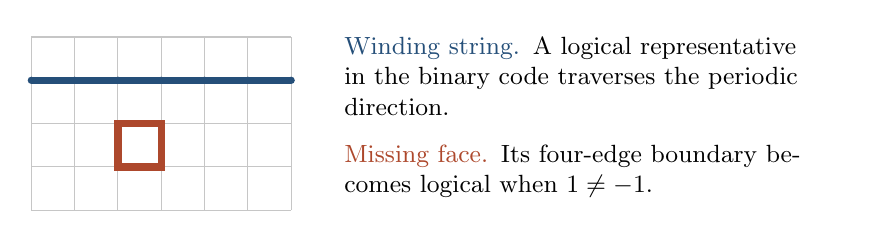
\begin{tikzpicture}[scale=.55]
\draw[step=1,gray!45] (0,0) grid (6,4);
\draw[blueink,line width=2.6pt] (0,3)--(6,3);
\foreach \x in {0,...,6} {\fill[blueink] (\x,3) circle (2.4pt);}
\draw[redink,line width=2.6pt] (2,1) rectangle (3,2);
\node[anchor=west,align=left,text width=6.3cm,font=\small] at (7.0,3.1) {\textcolor{blueink}{Winding string.} A logical representative in the binary code traverses the periodic direction.};
\node[anchor=west,align=left,text width=6.3cm,font=\small] at (7.0,.9) {\textcolor{redink}{Missing face.} Its four-edge boundary becomes logical when $1\ne -1$.};
\end{tikzpicture}
\caption{A patch of the periodic lattice, with the left and right edges identified. The placement of the omitted face is translated for visibility. The binary string spans one period. The support of the higher-dimensional logical operator is independent of the period.}
\end{figure}

\section{A support test for a proposed lift}
\begin{prop}\label{prop:count}
Let $G$ be an integer check matrix with isotropic image modulo $m$. For a set $S$ of physical sites, retain both labels per site in $G_S$. Write $N_m(M)$ for the size of the row image of $M$ over $R_m$. The number of distinct logical labels representable on $S$, including the identity, is
\begin{equation}\label{eq:count}
 |\mathcal L_m(S)|=
 \frac{m^{2|S|}\,N_m(G_{S^c})}{N_m(G_S)\,N_m(G)}.
\end{equation}
If $s_1,\ldots,s_t$ are the nonzero Smith invariants of $M$, then $N_m(M)=\prod_i m/\gcd(m,s_i)$.
\end{prop}
\begin{proof}
Let $V_S$ be the labels supported on $S$. The symplectic pairing on $V_S$ is perfect under the character $x\mapsto \exp(2\pi i x/m)$. The annihilator of the restricted stabilizer consequently has cardinality $m^{2|S|}/N_m(G_S)$. This is $|C^\perp\cap V_S|$. Projecting $C$ to $S^c$ gives $|C\cap V_S|=N_m(G)/N_m(G_{S^c})$. Taking the quotient gives Eq.~\eqref{eq:count}. Unimodular Smith operations are invertible modulo $m$, and multiplication by $s_i$ has image size $m/\gcd(m,s_i)$.
\end{proof}
Over a field $F$, the corresponding dimension is
\[
 \ell_F(S)=2|S|-\rank_F G_S-\rank_F G+\rank_F G_{S^c}.
\]
This dimension formula also appears in the proof of Theorem 12 of \cite{ldi26}. Over all sufficiently large primes, all ranks in this finite collection agree with their characteristic-zero values. Hence the eventual distance of a fixed integral lift with positive logical dimension is its rational symplectic quotient distance. To guarantee $d_p\ge d_2$ for all sufficiently large primes one must have $\ell_{\Q}(S)=0$ for every $|S|<d_2$; this condition is sufficient as well. A binary stabilizer can cease to be generated on $S$ even when the local syndrome rank is preserved. For the last two sites of Theorem~\ref{thm:seven}, $\rank G_S=3$ over both fields. The complementary rank rises from five over $\F_2$ to six over $\Q$, creating exactly one logical direction. This locates the failure directly in the quotient defining distance.

\section{Verification and scope}
The Lean project uses Lean 4.28.0 and a pinned revision of mathlib. It defines physical site weight using pairs of Pauli coordinates and distinguishes the full commuting module from the generated checks. The stand-alone theorem \texttt{distance\_collapse\_examples} combines the exact distances of the five-, seven- and eight-site codes. The project also proves freeness and reduction for Theorem~\ref{thm:five}, the integer triangular correction for Theorem~\ref{thm:seven}, and the displayed centered CSS rule in the eight-site case.

For Theorem~\ref{thm:lattice}, the code proves the binary distance for variable $L$, the rank and size of the pinned modules, and reduction from $\Z/4$ to the binary code. The main theorem in \texttt{UniversalTorus} compares the exact distances for every $L\ge4$ and $m>2$. One proof step transfers a nonzero kernel word on a signed incidence matrix to a binary word with support contained in its support. For Theorem~\ref{thm:css}, \texttt{CanonicalCycle} verifies the obstruction for arbitrary other matrix columns, given the specified cycle and ancillary-column restrictions. The existence of a dual tree realizing those restrictions on the torus is proved in the text. The field version of Proposition~\ref{prop:count} and its logical-existence criterion are formalized in \texttt{SupportRank}. The finite-ring counting formula, its Smith evaluation, and the code-space projector argument are proved in the text.

The sources were compiled and replayed by the Lean distribution's \texttt{leanchecker} with the pinned imports. The archive includes the transcripts, source hashes and three independent elementary Python calculations. Kernel verification establishes the stated algebraic implications. Interpretation of the published algorithms and priority require review of the original works. This manuscript is a research draft.
\begin{thebibliography}{10}
\bibitem{glp} H. Gluesing-Luerssen and T. Pllaha, On quantum stabilizer codes derived from local Frobenius rings, \emph{Finite Fields Appl.} \textbf{58}, 145--173 (2019). \href{https://doi.org/10.1016/j.ffa.2019.04.004}{doi:10.1016/j.ffa.2019.04.004}. \href{https://arxiv.org/abs/1710.09884}{arXiv:1710.09884}.
\bibitem{ldi20} L. G. Gunderman, Local-dimension-invariant qudit stabilizer codes, \emph{Phys. Rev. A} \textbf{101}, 052343 (2020). \href{https://doi.org/10.1103/PhysRevA.101.052343}{doi:10.1103/PhysRevA.101.052343}.
\bibitem{ldi22} L. G. Gunderman, Degenerate local-dimension-invariant stabilizer codes and an alternative bound for the distance preservation condition, \emph{Phys. Rev. A} \textbf{105}, 042424 (2022). \href{https://doi.org/10.1103/PhysRevA.105.042424}{doi:10.1103/PhysRevA.105.042424}. \href{https://arxiv.org/abs/2110.15274}{arXiv:2110.15274}.
\bibitem{ldi25} L. G. Gunderman, Beyond integral-domain stabilizer codes, \emph{Phys. Rev. A} \textbf{112}, 062430 (2025). \href{https://doi.org/10.1103/4y6f-xx6s}{doi:10.1103/4y6f-xx6s}. \href{https://arxiv.org/abs/2501.04888v1}{arXiv:2501.04888v1}.
\bibitem{ldi26} M. S. Islam, A. Reza and L. G. Gunderman, Local-dimension-invariant low-density parity-check stabilizer codes, preprint (2026). \href{https://arxiv.org/abs/2610.15893}{arXiv:2610.15893v1}.
\bibitem{kitaev} A. Yu. Kitaev, Fault-tolerant quantum computation by anyons, \emph{Ann. Phys.} \textbf{303}, 2--30 (2003). \href{https://doi.org/10.1016/S0003-4916(02)00018-0}{doi:10.1016/S0003-4916(02)00018-0}.
\bibitem{dk} E. Dennis, A. Kitaev, A. Landahl and J. Preskill, Topological quantum memory, \emph{J. Math. Phys.} \textbf{43}, 4452--4505 (2002). \href{https://doi.org/10.1063/1.1499754}{doi:10.1063/1.1499754}.
\bibitem{wcf} H. Watanabe, M. Cheng and Y. Fuji, Ground state degeneracy on torus in a family of $\mathbb Z_N$ toric code, \emph{J. Math. Phys.} \textbf{64}, 051901 (2023). \href{https://doi.org/10.1063/5.0134010}{doi:10.1063/5.0134010}.
\bibitem{pith} Pith, Machine review of arXiv:2610.15893v1 (14 October 2026), objection concerning Eqs.~(16)--(17). \url{https://pith.science/paper/2610.15893}.
\end{thebibliography}
\end{document}
